% Created 2024-10-16 śro 21:35
% Intended LaTeX compiler: pdflatex
\documentclass[../../main.tex]{subfiles}

% \usepackage[a4paper, margin=3cm]{geometry}
% \usepackage{amssymb} // not working

\usepackage[T1]{fontenc}
\usepackage[utf8]{inputenc}
\usepackage{graphicx}
\usepackage{longtable}
\usepackage{wrapfig}
\usepackage{rotating}
\usepackage[normalem]{ulem}
\usepackage{amsmath}
\usepackage{capt-of}
\usepackage{hyperref}
\usepackage{siunitx}
\usepackage{float}
\usepackage[polish]{babel}

\graphicspath{{../}}
\author{Wojciech Paderewski}
\date{\today}
\title{Koncepcja ukladu}
\hypersetup{
 pdfauthor={Wojciech Paderewski},
 pdftitle={Koncepcja ukladu},
 pdfkeywords={},
 pdfsubject={},
 pdflang={Polish}}

\begin{document}

\subsubsection{Dobór złącza}
W doborze złącza kluczowe kluczowa była jego wielkość oraz prąd, który jest w stanie przewodzić. Teoretyczna moc układu to 10W,
co przy napięciu 12V daje prąd 0.83A. Złącze musi być w stanie przewodzić prąd 1.5A, by zapewnić bezpieczeństwo. 

Wybrano złącze firmy same sky o symbolu PJ-094H-SMT-TR o styku 0.65x2.35mm, które jest w stanie przewodzić prąd 2.5A, czyli więcej niż wystarczająco.
Złącze jest bardzo niskie, jego wysokość to 3.5mm, co pozwala na zminimalizowanie wysokości zegara.
\subsubsection{Opis podłączenia}
Jako kondensatory filtrujące wykorzystano, 2 kondensatory o 
pojemności 100uF w celu zminimalizowania zakłóceń niskich częstotliwości, oraz 1 kondensator o pojemności 100nF w celu zminimalizowania zakłóceń wysokich częstotliwości.

Kondensatory 100uF są kondensatorami tantalowymi, a kondensator 100nF jest kondensatorem ceramicznym. Wykorzystano te rodzaje kondensatorów, 
ponieważ są to kondensatory o długiej żywotności, a także są to kondensatory o małych rozmiarach w przeciwieństwie do kondensatorów elektrolitycznych.
\subsubsection{Zabezpieczenia ESD}
W celu zabezpieczenia linii przed przepięciami, wykorzystano diodę TVS firmy Wurth Elektronik o symbolu 824045812. Dioda ta jest diodą TVS o napięciu przebicia 13.3V,
oraz napięciu stabilizacji 15V. Dioda musi mieć jak najmniejsze napięcie przebicia, by skok napięcia nie uszkodził rejestrów przesuwnych HV, które są wrażliwe na napięcia powyżej 13.2V.

Dioda ta została wybrana gdyż nie udało się znaleźć diody TVS o napięciu stabilizacji 13V. Ma ona również dużą pojemność, co powoduje, że nie jest ona zalecana do 
zastosowań z wysokimi częstotliwościami, jednak w tym przypadku nie jest to problemem, gdyż jest to tylko złącze zasilania o stałym napięciu.
\subsubsection{Schemat}
\begin{figure}[H]
    \centering
    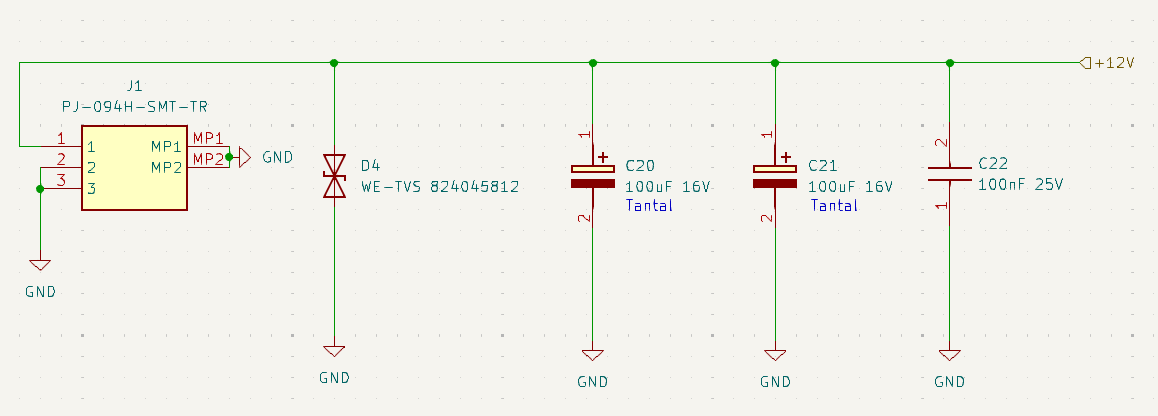
\includegraphics[width=0.8\textwidth]{DcPlug_schemat.png}
    \caption{Schemat złącza DC-Plug}
\end{figure}

\end{document}
